\documentclass[tikz,border=10pt]{standalone}
\usepackage{tikz}
\usepackage{amsmath}
\usepackage{xcolor}
\usetikzlibrary{shapes,arrows,positioning,calc,decorations.pathreplacing,fit,shadows,patterns,chains}

% Define colors
\definecolor{blockchain}{RGB}{255, 140, 0}
\definecolor{security}{RGB}{220, 20, 60}
\definecolor{transparency}{RGB}{30, 144, 255}
\definecolor{consensus}{RGB}{50, 205, 50}
\definecolor{citizen}{RGB}{138, 43, 226}
\definecolor{background}{RGB}{248, 249, 250}

\begin{document}
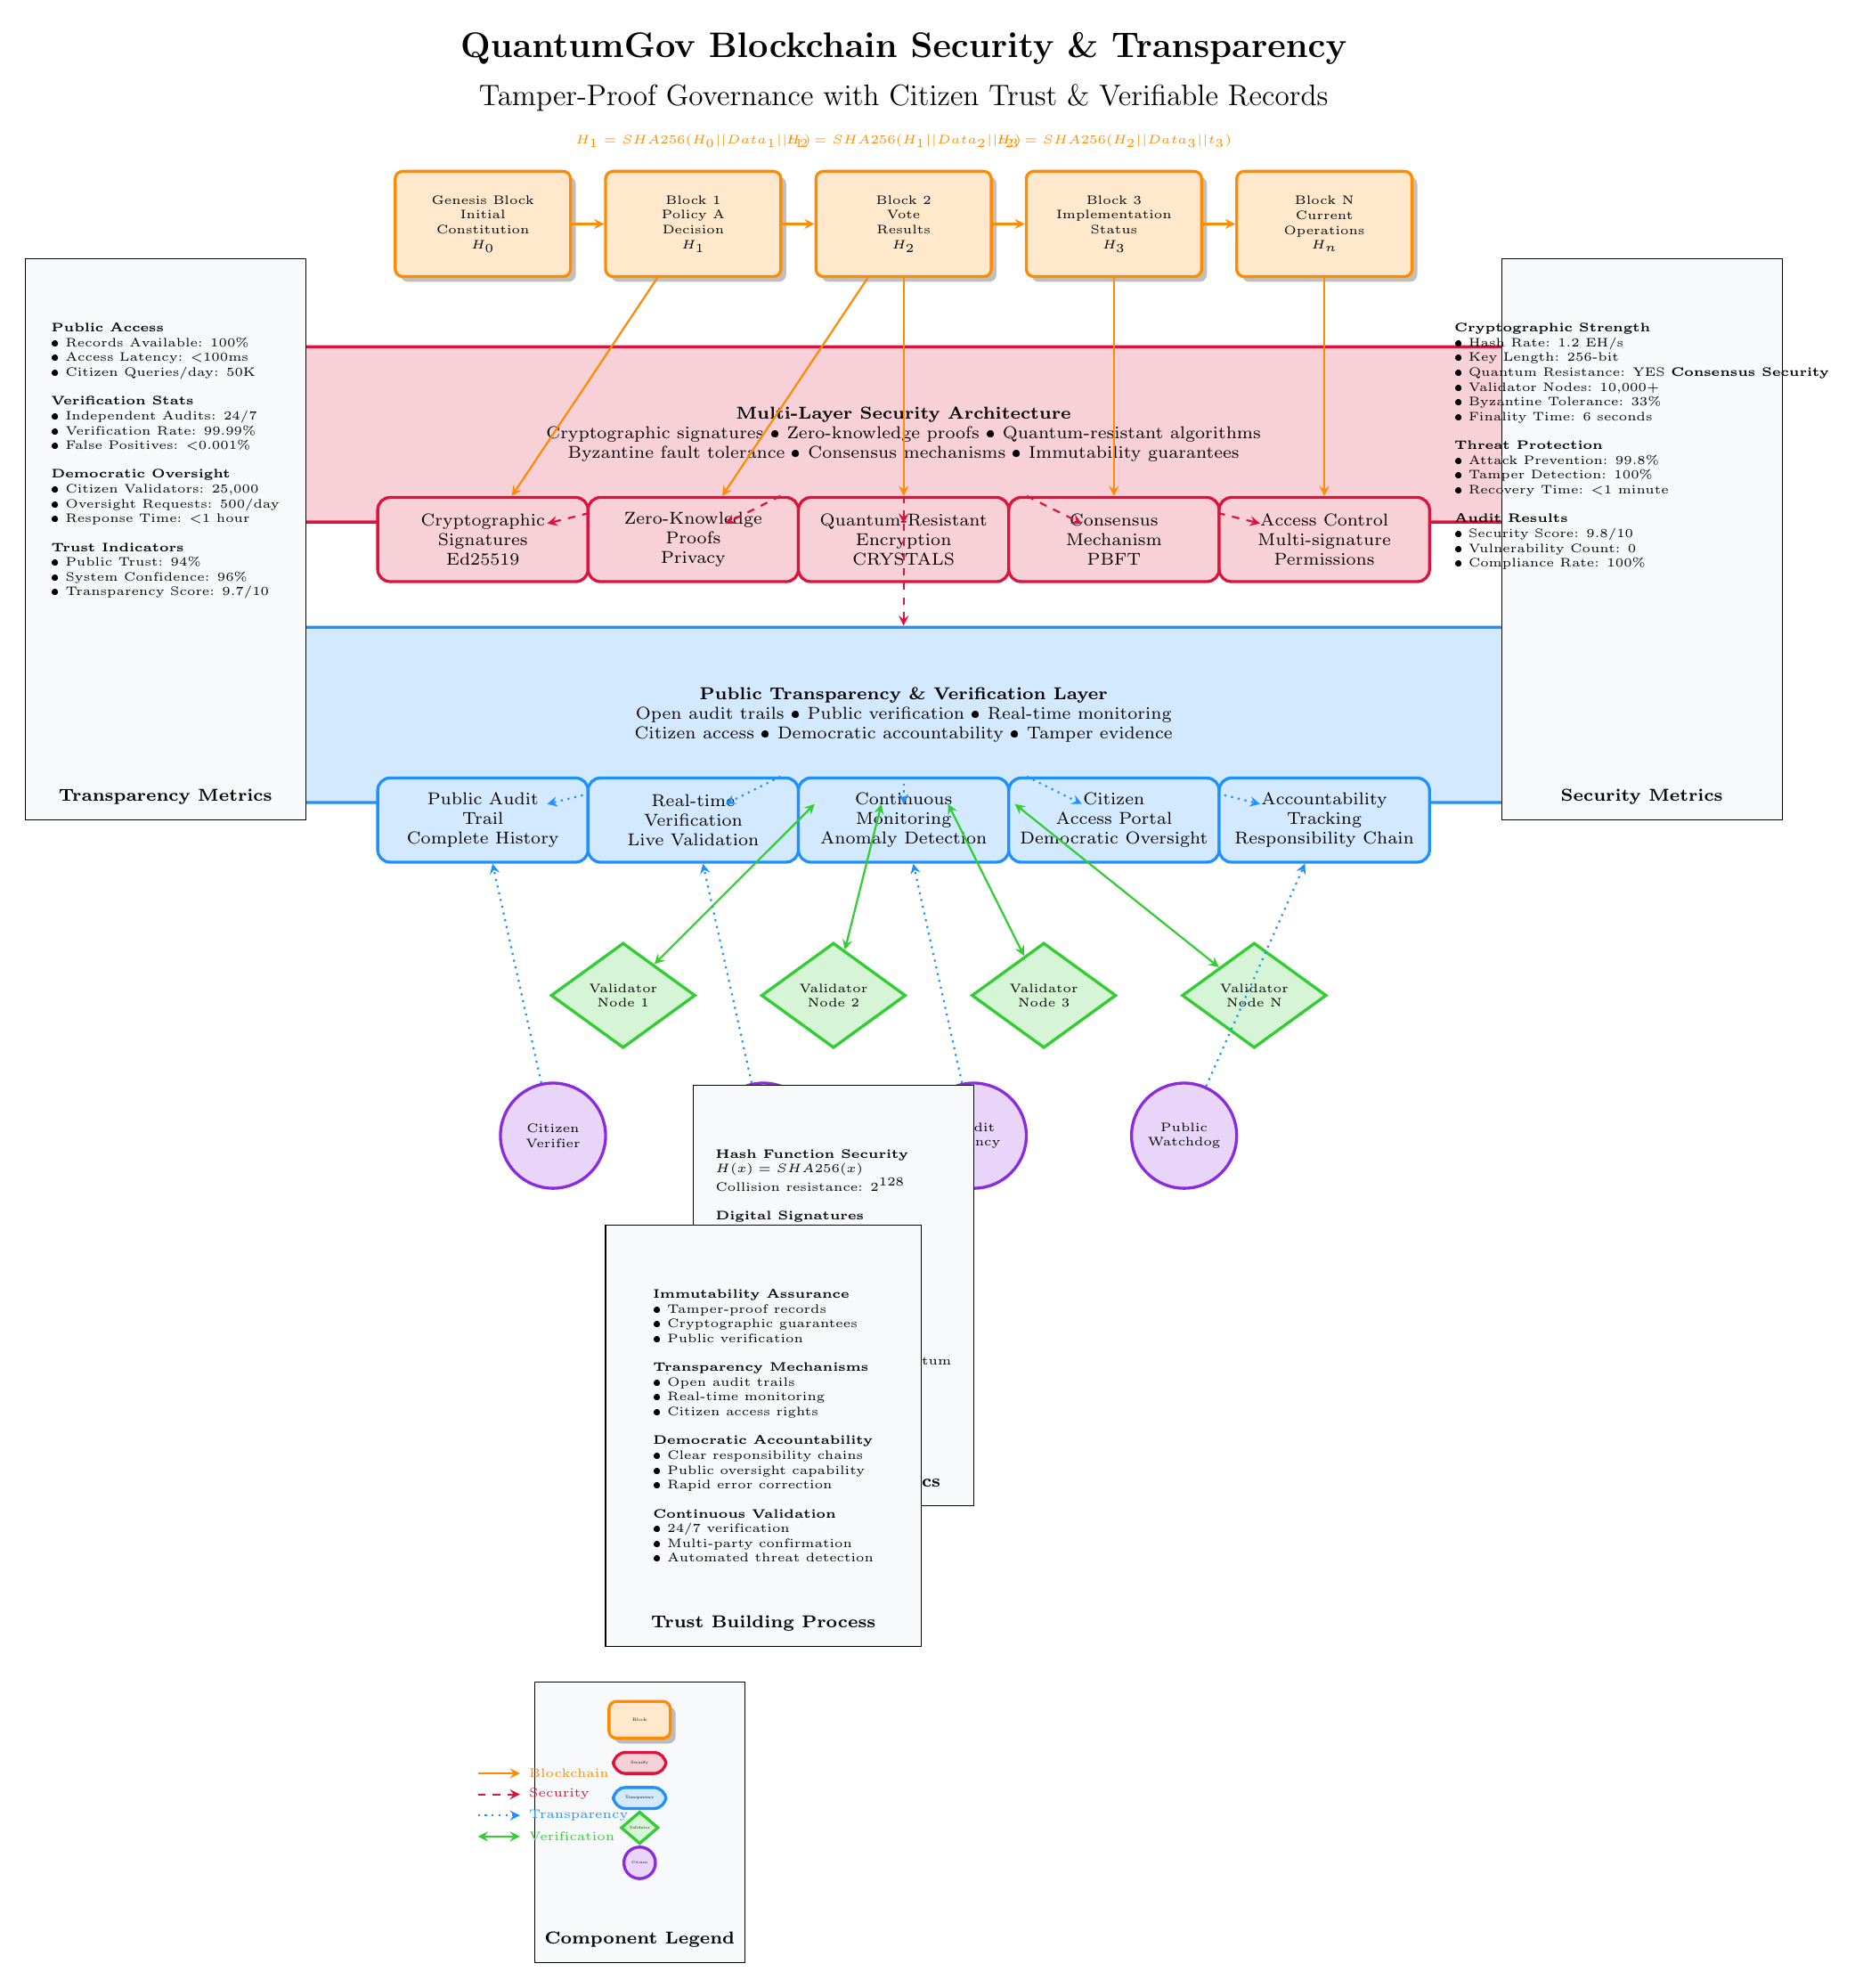
\begin{tikzpicture}[
    node distance=1cm,
    block/.style={rectangle, rounded corners=3pt, draw=blockchain, fill=blockchain!20, minimum height=1.5cm, minimum width=2.5cm, align=center, font=\tiny, very thick, drop shadow},
    security_node/.style={rectangle, rounded corners=5pt, draw=security, fill=security!20, minimum height=1.2cm, minimum width=3cm, align=center, font=\scriptsize, very thick},
    transparency_node/.style={rectangle, rounded corners=5pt, draw=transparency, fill=transparency!20, minimum height=1.2cm, minimum width=3cm, align=center, font=\scriptsize, very thick},
    citizen_node/.style={circle, draw=citizen, fill=citizen!20, minimum size=1.5cm, align=center, font=\tiny, very thick},
    validator_node/.style={diamond, draw=consensus, fill=consensus!20, minimum size=1.5cm, align=center, font=\tiny, very thick, aspect=1.5},
    chain/.style={->, thick, >=stealth, color=blockchain},
    security_flow/.style={->, thick, >=stealth, color=security, dashed},
    transparency_flow/.style={->, thick, >=stealth, color=transparency, dotted},
    verification/.style={<->, thick, >=stealth, color=consensus}
]

% Title
\node[align=center, font=\Large\bfseries] at (0, 16) {QuantumGov Blockchain Security \& Transparency};
\node[align=center, font=\large] at (0, 15.3) {Tamper-Proof Governance with Citizen Trust \& Verifiable Records};

% Blockchain Chain (Top)
\node[block] (genesis) at (-6, 13.5) {Genesis Block\\Initial\\Constitution\\$H_0$};
\node[block] (block1) at (-3, 13.5) {Block 1\\Policy A\\Decision\\$H_1$};
\node[block] (block2) at (0, 13.5) {Block 2\\Vote\\Results\\$H_2$};
\node[block] (block3) at (3, 13.5) {Block 3\\Implementation\\Status\\$H_3$};
\node[block] (blockn) at (6, 13.5) {Block N\\Current\\Operations\\$H_n$};

% Chain connections
\draw[chain] (genesis) -- (block1);
\draw[chain] (block1) -- (block2);
\draw[chain] (block2) -- (block3);
\draw[chain] (block3) -- (blockn);

% Hash formulas above blocks
\node[above=0.2cm of block1, font=\tiny, color=blockchain] {$H_1 = SHA256(H_0 || Data_1 || t_1)$};
\node[above=0.2cm of block2, font=\tiny, color=blockchain] {$H_2 = SHA256(H_1 || Data_2 || t_2)$};
\node[above=0.2cm of block3, font=\tiny, color=blockchain] {$H_3 = SHA256(H_2 || Data_3 || t_3)$};

% Security Layer (Middle)
\node[security_node, minimum width=18cm, minimum height=2.5cm] (security_layer) at (0, 10.5) {
    \textbf{Multi-Layer Security Architecture}\\
    Cryptographic signatures • Zero-knowledge proofs • Quantum-resistant algorithms\\
    Byzantine fault tolerance • Consensus mechanisms • Immutability guarantees
};

% Security Components
\node[security_node] (crypto) at (-6, 9) {Cryptographic\\Signatures\\Ed25519};
\node[security_node] (zkp) at (-3, 9) {Zero-Knowledge\\Proofs\\Privacy};
\node[security_node] (quantum_resist) at (0, 9) {Quantum-Resistant\\Encryption\\CRYSTALS};
\node[security_node] (consensus_mech) at (3, 9) {Consensus\\Mechanism\\PBFT};
\node[security_node] (access_control) at (6, 9) {Access Control\\Multi-signature\\Permissions};

% Transparency Layer (Middle-Bottom)
\node[transparency_node, minimum width=18cm, minimum height=2.5cm] (transparency_layer) at (0, 6.5) {
    \textbf{Public Transparency \& Verification Layer}\\
    Open audit trails • Public verification • Real-time monitoring\\
    Citizen access • Democratic accountability • Tamper evidence
};

% Transparency Components
\node[transparency_node] (audit_trail) at (-6, 5) {Public Audit\\Trail\\Complete History};
\node[transparency_node] (verification) at (-3, 5) {Real-time\\Verification\\Live Validation};
\node[transparency_node] (monitoring) at (0, 5) {Continuous\\Monitoring\\Anomaly Detection};
\node[transparency_node] (citizen_access) at (3, 5) {Citizen\\Access Portal\\Democratic Oversight};
\node[transparency_node] (accountability) at (6, 5) {Accountability\\Tracking\\Responsibility Chain};

% Validator Network (Bottom)
\node[validator_node] (validator1) at (-4, 2.5) {Validator\\Node 1};
\node[validator_node] (validator2) at (-1, 2.5) {Validator\\Node 2};
\node[validator_node] (validator3) at (2, 2.5) {Validator\\Node 3};
\node[validator_node] (validator4) at (5, 2.5) {Validator\\Node N};

% Citizen Network (Bottom)
\node[citizen_node] (citizen1) at (-5, 0.5) {Citizen\\Verifier};
\node[citizen_node] (citizen2) at (-2, 0.5) {Oversight\\Committee};
\node[citizen_node] (citizen3) at (1, 0.5) {Audit\\Agency};
\node[citizen_node] (citizen4) at (4, 0.5) {Public\\Watchdog};

% Security Connections
\draw[security_flow] (crypto) -- (security_layer);
\draw[security_flow] (zkp) -- (security_layer);
\draw[security_flow] (quantum_resist) -- (security_layer);
\draw[security_flow] (consensus_mech) -- (security_layer);
\draw[security_flow] (access_control) -- (security_layer);

% Transparency Connections
\draw[transparency_flow] (audit_trail) -- (transparency_layer);
\draw[transparency_flow] (verification) -- (transparency_layer);
\draw[transparency_flow] (monitoring) -- (transparency_layer);
\draw[transparency_flow] (citizen_access) -- (transparency_layer);
\draw[transparency_flow] (accountability) -- (transparency_layer);

% Blockchain to Security
\draw[chain] (block1) -- (crypto);
\draw[chain] (block2) -- (zkp);
\draw[chain] (block2) -- (quantum_resist);
\draw[chain] (block3) -- (consensus_mech);
\draw[chain] (blockn) -- (access_control);

% Security to Transparency
\draw[security_flow] (security_layer) -- (transparency_layer);

% Validator Verification
\draw[verification] (validator1) -- (transparency_layer);
\draw[verification] (validator2) -- (transparency_layer);
\draw[verification] (validator3) -- (transparency_layer);
\draw[verification] (validator4) -- (transparency_layer);

% Citizen Verification
\draw[transparency_flow] (citizen1) -- (audit_trail);
\draw[transparency_flow] (citizen2) -- (verification);
\draw[transparency_flow] (citizen3) -- (monitoring);
\draw[transparency_flow] (citizen4) -- (accountability);

% Security Metrics Panel
\node[draw, fill=background, minimum width=4cm, minimum height=8cm, right=1cm of access_control] (security_metrics) {};
\node[above=0.1cm of security_metrics.south, font=\scriptsize\bfseries, align=center] {Security Metrics};
\node[below=0.8cm of security_metrics.north, font=\tiny, align=left] {
    \textbf{Cryptographic Strength}\\
    • Hash Rate: 1.2 EH/s\\
    • Key Length: 256-bit\\
    • Quantum Resistance: YES
    \textbf{Consensus Security}\\
    • Validator Nodes: 10,000+\\
    • Byzantine Tolerance: 33\%\\
    • Finality Time: 6 seconds\\[0.2cm]
    \textbf{Threat Protection}\\
    • Attack Prevention: 99.8\%\\
    • Tamper Detection: 100\%\\
    • Recovery Time: <1 minute\\[0.2cm]
    \textbf{Audit Results}\\
    • Security Score: 9.8/10\\
    • Vulnerability Count: 0\\
    • Compliance Rate: 100\%
};

% Transparency Metrics Panel
\node[draw, fill=background, minimum width=4cm, minimum height=8cm, left=1cm of crypto] (transparency_metrics) {};
\node[above=0.1cm of transparency_metrics.south, font=\scriptsize\bfseries, align=center] {Transparency Metrics};
\node[below=0.8cm of transparency_metrics.north, font=\tiny, align=left] {
    \textbf{Public Access}\\
    • Records Available: 100\%\\
    • Access Latency: <100ms\\
    • Citizen Queries/day: 50K\\[0.2cm]
    \textbf{Verification Stats}\\
    • Independent Audits: 24/7\\
    • Verification Rate: 99.99\%\\
    • False Positives: <0.001\%\\[0.2cm]
    \textbf{Democratic Oversight}\\
    • Citizen Validators: 25,000\\
    • Oversight Requests: 500/day\\
    • Response Time: <1 hour\\[0.2cm]
    \textbf{Trust Indicators}\\
    • Public Trust: 94\%\\
    • System Confidence: 96\%\\
    • Transparency Score: 9.7/10
};

% Mathematical Framework Panel
\node[draw, fill=background, minimum width=4cm, minimum height=6cm, below=0.5cm of validator2] (math_panel) {};
\node[above=0.1cm of math_panel.south, font=\scriptsize\bfseries, align=center] {Security Mathematics};
\node[below=0.8cm of math_panel.north, font=\tiny, align=left] {
    \textbf{Hash Function Security}\\
    $H(x) = SHA256(x)$\\
    Collision resistance: $2^{128}$\\[0.2cm]
    \textbf{Digital Signatures}\\
    $Verify(PK, m, \sigma) = true$\\
    $(sk, pk) \leftarrow KeyGen()$\\[0.2cm]
    \textbf{Consensus Probability}\\
    $P(Byzantine) < \frac{1}{3}$\\
    Safety: $P(fork) < 10^{-12}$\\[0.2cm]
    \textbf{Quantum Resistance}\\
    $Security \geq 2^{256}$ post-quantum
};

% Trust Building Process Panel
\node[draw, fill=background, minimum width=4.5cm, minimum height=6cm, below=0.5cm of citizen2] (trust_panel) {};
\node[above=0.1cm of trust_panel.south, font=\scriptsize\bfseries, align=center] {Trust Building Process};
\node[below=0.8cm of trust_panel.north, font=\tiny, align=left] {
    \textbf{Immutability Assurance}\\
    • Tamper-proof records\\
    • Cryptographic guarantees\\
    • Public verification\\[0.2cm]
    \textbf{Transparency Mechanisms}\\
    • Open audit trails\\
    • Real-time monitoring\\
    • Citizen access rights\\[0.2cm]
    \textbf{Democratic Accountability}\\
    • Clear responsibility chains\\
    • Public oversight capability\\
    • Rapid error correction\\[0.2cm]
    \textbf{Continuous Validation}\\
    • 24/7 verification\\
    • Multi-party confirmation\\
    • Automated threat detection
};

% Legend
\node[draw, fill=background, minimum width=3cm, minimum height=4cm, below left=0.5cm and -2cm of trust_panel] (legend) {};
\node[above=0.1cm of legend.south, font=\scriptsize\bfseries, align=center] {Component Legend};
\node[block, scale=0.35, above=3.2cm of legend.south] (leg_block) {Block};
\node[security_node, scale=0.25, above=2.7cm of legend.south] (leg_security) {Security};
\node[transparency_node, scale=0.25, above=2.2cm of legend.south] (leg_transparency) {Transparency};
\node[validator_node, scale=0.3, above=1.7cm of legend.south] (leg_validator) {Validator};
\node[citizen_node, scale=0.3, above=1.2cm of legend.south] (leg_citizen) {Citizen};

% Flow Legend
\draw[chain] (legend.west) ++(-0.8, 0.7) -- ++(0.6, 0) node[right, font=\tiny] {Blockchain};
\draw[security_flow] (legend.west) ++(-0.8, 0.4) -- ++(0.6, 0) node[right, font=\tiny] {Security};
\draw[transparency_flow] (legend.west) ++(-0.8, 0.1) -- ++(0.6, 0) node[right, font=\tiny] {Transparency};
\draw[verification] (legend.west) ++(-0.8, -0.2) -- ++(0.6, 0) node[right, font=\tiny] {Verification};

\end{tikzpicture}
\end{document}